%!TEX TS-program = Xelatex  
%!TEX encoding = UTF-8 Unicode  
  
  
\documentclass[12pt]{article}  
\usepackage{geometry}  
\geometry{letterpaper}  
  
\usepackage{fancyhdr} 
\usepackage{layout}
\addtolength{\hoffset}{-1.0cm} \addtolength{\textwidth}{2cm}
\addtolength{\voffset}{-1.0cm} \addtolength{\textheight}{2cm}
\usepackage[rgb]{xcolor}

\usepackage{cite}
\makeatletter
\def\@cite#1#2{\textsuperscript{[{#1\if@tempswa , #2\fi}]}}
\makeatother

\usepackage{listings}
\definecolor{dkgreen}{rgb}{0,0.6,0}
\definecolor{gray}{rgb}{0.5,0.5,0.5}
\definecolor{bcol}{rgb}{0.85,0.85,0.85}
\definecolor{mauve}{rgb}{0.58,0,0.82}
\definecolor{mygray}{gray}{.9}
\definecolor{mypink}{rgb}{.99,.91,.95}
\definecolor{mycyan}{cmyk}{.3,0,0,0}

\lstset{ %
language=python,                % the language of the code
basicstyle=\footnotesize,       % the size of the fonts that are used for the code
numbers=left,                   % where to put the line-numbers
numberstyle=\tiny\color{gray},  % the style that is used for the line-numbers
stepnumber=1,                   % the step between two line-numbers. If it's 1, each line
                                % will be numbered
numbersep=5pt,                  % how far the line-numbers are from the code
backgroundcolor=\color{bcol},   % choose the background color. You must add \usepackage{color}
showspaces=false,               % show spaces adding particular underscores
showstringspaces=false,         % underline spaces within strings
showtabs=false,                 % show tabs within strings adding particular underscores
frame=shadowbox,                % adds a frame around the code
rulecolor=\color{black},        % if not set, the frame-color may be changed on line-breaks within not-black text (e.g. commens (green here))
tabsize=2,                      % sets default tabsize to 2 spaces
captionpos=t,                   % sets the caption-position to bottom
breaklines=true,                % sets automatic line breaking
breakatwhitespace=false,        % sets if automatic breaks should only happen at whitespace
title=\lstname,                     % show the filename of files included with \lstinputlisting;
                                    % also try caption instead of title
keywordstyle=\color{blue},          % keyword style
commentstyle=\color{dkgreen},       % comment style
stringstyle=\color{mauve},          % string literal style
escapeinside=``,                    % if you want to add LaTeX within your code
morekeywords={LONG64,LONGLONG,bool}                % if you want to add more keywords to the set
}



\usepackage{flushend, cuted} %

\usepackage{indentfirst,latexsym,bm}
\usepackage{amsmath,amssymb,amsfonts}
\usepackage{pifont} 
\usepackage{fontspec,xltxtra,xunicode}  
\defaultfontfeatures{Mapping=tex-text}  

\usepackage{algorithmic}
\usepackage[noend, ruled, linesnumbered]{algorithm2e}
\setromanfont{华文宋体} %设置中文字体  
\XeTeXlinebreaklocale “zh”  
\XeTeXlinebreakskip = 0pt plus 1pt minus 0.1pt %文章内中文自动换行  
  
 \setlength{\columnsep}{3em}          %设置分栏间隔
\setlength{\parindent}{2em}          %设置段首缩进量
\renewcommand{\baselinestretch}{1.2} %重设行距     
 \usepackage{graphicx}
\usepackage{cite}
\newcommand{\red}[1]{  \textcolor{red}  {#1}}   %红色\makeatletter
\newcommand{\blue}[1]{ \textcolor{blue} {#1}}   %蓝色\def\@cite#1#2{\textsuperscript{[{#1\if@tempswa , #2\fi}]}}
\newcommand{\green}[1]{\textcolor{green}{#1}}   %绿色\makeatother


% ----------------------------------------------------------------
\vfuzz2pt % Don't report over-full v-boxes if over-edge is small
\hfuzz2pt % Don't report over-full h-boxes if over-edge is small

%%--------------------------------------------------
%% 图片文件路径
%%--------------------------------------------------
\graphicspath{{Figures/}}


% MATH -----------------------------------------------------------
\DeclareMathOperator{\diag}{diag}
\DeclareMathOperator{\rank}{rank}
\DeclareMathOperator{\vecm}{vec}
\DeclareMathOperator{\vecs}{vecs}

\newcommand{\mfloor}[1]{ \left\lfloor {#1} \right\rfloor }
\newcommand{\mpair}[2]{ \left\langle {#1}, {#2} \right\rangle}


\renewcommand{\bf}[1]{\mathbf{#1}}
\renewcommand{\vec}[1]{\bm{#1}}    %向量, 黑斜体
\newcommand{\mat}[1]{\bm{#1}}    %矩阵
\newcommand{\dif}{\mathrm{d}}
\newcommand{\me} {\mathrm{e}}
\newcommand{\mi} {\mathrm{i}}
\newcommand{\vei} {\mathrm{vec}}

\newcommand{\vecmat}[1]{\vecm{\left( #1 \right)}}
\newcommand{\vecsmat}[1]{\vecs{\left( #1 \right)}}
\newcommand{\vecasym}[1]{[#1]_\times}   % antisymmetric matrix from a vector
\newcommand{\id} {\mathbbm{1}}   % identity operator
\newcommand{\fracode}[2]{\frac{\dif {#1}}{\dif {#2}}}         % ordinary differential operator
\newcommand{\fracpde}[2]{\frac{\partial {#1}}{\partial {#2}}} % partial differential operator
\newcommand{\fracpderow}[2]{\partial {#1}/\partial {#2}}
\newcommand{\fracoderow}[2]{\dif {#1}/\dif {#2}}
\newcommand{\fracpdemix}[3]{\frac{\partial^2 {#1}}{\partial {#2} \partial {#3}}}
\newcommand{\lap}[2]{\frac{\partial^2 {#1}}{\partial {#2}^2}}
\newcommand{\laprow}[2]{\partial^2 {#1}/\partial {#2}^2}
\newcommand{\secode}[2]{\frac{\dif^2 {#1}}{\dif {#2}^2}}
\newcommand{\set}[1]{\left\{ #1 \right\}}
\newcommand{\abs}[1]{\left| #1 \right|}
\newcommand{\absvec}[1]{\left| \bf{#1} \right|}
\newcommand{\ket}[1]{|#1 \rangle}
\newcommand{\bra}[1]{\langle #1 |}
\newcommand{\braket}[2]{ \langle #1 | #2 \rangle}
\newcommand{\norm}[1]{\lVert #1 \rVert}
\newcommand{\normF}[1]{{\parallel #1 \parallel}_\textrm{F}}
\newcommand{\trsp}[1]{{#1}^\textsf{T}}
\newcommand{\inv}[1]{#1^{-1}}
\newcommand{\ginv}[1]{#1^+}    % Moore-Penrose (general) inverse
\newcommand{\tinv}[1]{{#1}^{-\textsf{T}}}


\newcommand{\ES}[3]{\mathbb{#1}^{{#2}\times {#3}}}               % Euclidean space
\newcommand{\PS}[3]{\mathbb{#1}^{{#2}\times{#3}}}      % projective space
% ----------------------------------------------------------------
\newfontfamily{\H}{微软雅黑}  
\newfontfamily{\E}{Arial}  


\newfontfamily{\TNR}{Times New Roman}  %设定新的字体快捷命令  
\title{{\H Weekly Report of Research Work\\ }\quad {WR-ABS-TEMP-2015A-No.007}}
\author{汤吉(Ji TANG)\\
               Number: WR-ABS-TEMP-2015A,  E-mail: tangji08@hotmail.com \\
        Date: 3/1/2016 - 10/1/2016}
        \date{January 10, 2016}

  
 %%*************************************************
%%  打印 标题, 作者, 日期等内容
%%*************************************************
\begin{document}  
\maketitle
%%*********************************************
%% 设置页眉与页脚
%%*********************************************
\pagestyle{fancy}
\fancyhead[LO,RE]{\leftmark} % clear all fields
\fancyhead[RO,LE]{WR-ABS-TEMP-2015A-No.007-TJx}   %  请设置正确的个人文档编号



\fancyfoot[LO,RE]{SIAE}
\fancyfoot[RO,RE]{Ji Tang}
\renewcommand{\headrulewidth}{0.4pt}
\renewcommand{\footrulewidth}{0.4pt}



%%*************************************************
%% 显示内容目录
%%*************************************************
\tableofcontents 
\newpage
%%*************************************************
%% 正文部分
%%*************************************************
\section{\H Work}
\begin{enumerate}
	\item I have learned something about machine learning.
	\item I have studied the international economic.
\end{enumerate}

\section{\H A real example in the book}
\subsection{\H Translate File to Matrix}
\subsubsection{Introduction}
In the book, Hellen has classified 3 kinds of persons:\\1.People she didn't like\\2.People she likes in small doses\\3.People she liked in large doses

And she has recorded the following features:\\1.Number of frequent flyer miles earned per year\\2.Percentage of time spent playing video games\\3.Liters of ice cream consumed per week

First of all, we need to change the data to the format that my classifier accepts. So we have to add a new function named "file2matrix"
\subsubsection{Code}
\begin{lstlisting}
def file2matrix(filename):
   fr = open(filename) #Load the data
   NumbersOfLines = len(fr.readlines()) #Get the number of the lines
   returnMatrix = zeros((NumbersOfLines, 3)) #Create Numpy matrix to return
   classLabelVector = []
   fr = open(filename) #Reload the data
   index = 0
   for line in fr.readlines():
      lines = line.strip() #strip the beginning and the end blank
      listFromLine = lines.split() #separate each line by '\t'
      returnMatrix[index,:] = listFromLine[0:3] #Get the 3 values of each line
      classLabelVector.append(int(listFromLine[-1])) #Get the evaluate of each person
      index += 1
   return returnMatrix, classLabelVector
\end{lstlisting}

\subsection{\H Plot the picture}
\subsubsection{Picture}
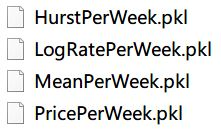
\includegraphics[width=5.5in]{1.jpg}
\subsubsection{Code}
\begin{lstlisting}
from numpy import *
import kNN
import matplotlib.pyplot as plt
datingDataMat, datingLabels = kNN.file2matrix('C:\Documents\Python\kNN\datingTestSet.txt')
color = ['r^','b*','g.'] #Set the color form
fig = plt.figure()
ax = fig.add_subplot(111)

for j in [1,2,3]:
    a = [i for i in range(len(datingLabels)) if datingLabels[i] == j] #Find out the person corresponding to 1,2,3
    b = [[datingDataMat[i][0],datingDataMat[i][1]] for i in a]
    c = array(b)
    plt.plot(c[:,0],c[:,1],color[j-1])
plt.xlabel('Frequent Flyier Miles Earned Per Year')
plt.ylabel('Percentage of Time Spent Playing Video Games')
plt.show()

\end{lstlisting}

\subsection{\H Normalizing numeric values}
\subsubsection{Introduction}
The largest term, the number of frequent flyer miles earned per year, will have the most effect. But it shouldn't have any extra importance, so dealing with values that lie in different ranges, it's common to normalize them. Common ranges to normalize them to are 0 to 1 or -1 to 1. To scale everything from 0 to 1, we need to apply the following formula
$$NewValue = \frac{OldValue - Min}{Max - Min}$$
\subsubsection{Code}
\begin{lstlisting}
def autoNorm(dataSet):
   minValues = dataSet.min(0) #The min value
   maxValues = dataSet.max(0) #The max value
   ranges = maxValues - minValues
   # normDataset = zeros(shape(dataSet)) 
   m = dataSet.shape[0] #The number of lines
   normDataset = dataSet - tile(minValues, (m, 1))
   normDataset = normDataset/tile(ranges, (m, 1)) #Calculate the values normalized
   return normDataset, ranges, minValues

\end{lstlisting}

\subsection{\H Set up the predictor}
\subsubsection{Code}
\begin{lstlisting}
def classifyPerson():
   resultList = ['not at all','in small doses','in large doses']
   ffMiles = float(raw_input("\nFrequent fliter miles earned per year?\n"))
   percentage = float(\raw_input("Percentage of time spent playing video games?matrix\n"))
   iceCream = float(raw_input("\nLiters of ice cream consumed per year?\n"))
   datingDataMat, datingLabels = file2matrix('C:\Documents\Python\kNN\datingTestSet.txt')
   normMat, ranges, minValues = autoNorm(datingDataMat)
   inArr = array([ffMiles, percentage, iceCream])
   classifiedReasult = classify((inArr-minValues)/ranges, normMat, datingLabels, 10)
   print "You will probably like this person:", resultList[classifiedReasult - 1]

\end{lstlisting}

\subsection{\H Result}
Then I have selected 3 samples randomly and have tested them.

\H{Sample 1:}

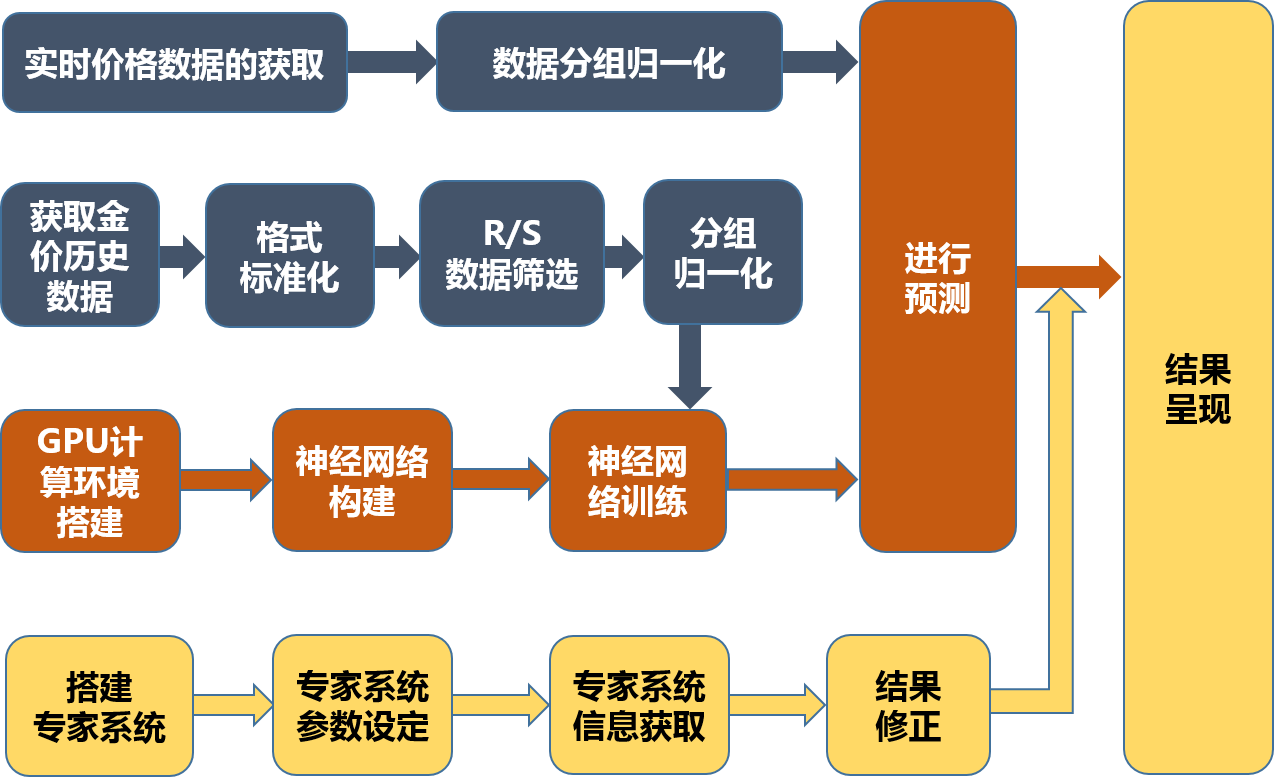
\includegraphics[width=5.5in]{3.jpg}

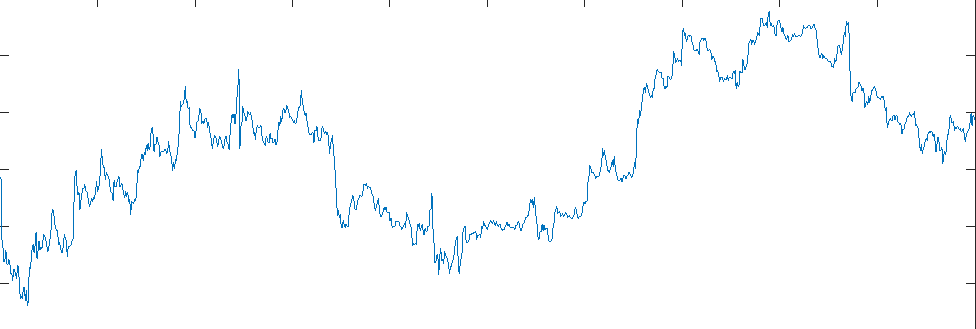
\includegraphics[width=5.5in]{2.jpg}

\H{Sample 2:}

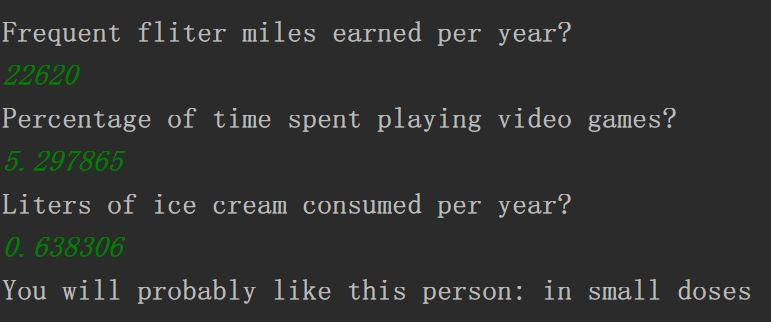
\includegraphics[width=5.5in]{5.jpg}

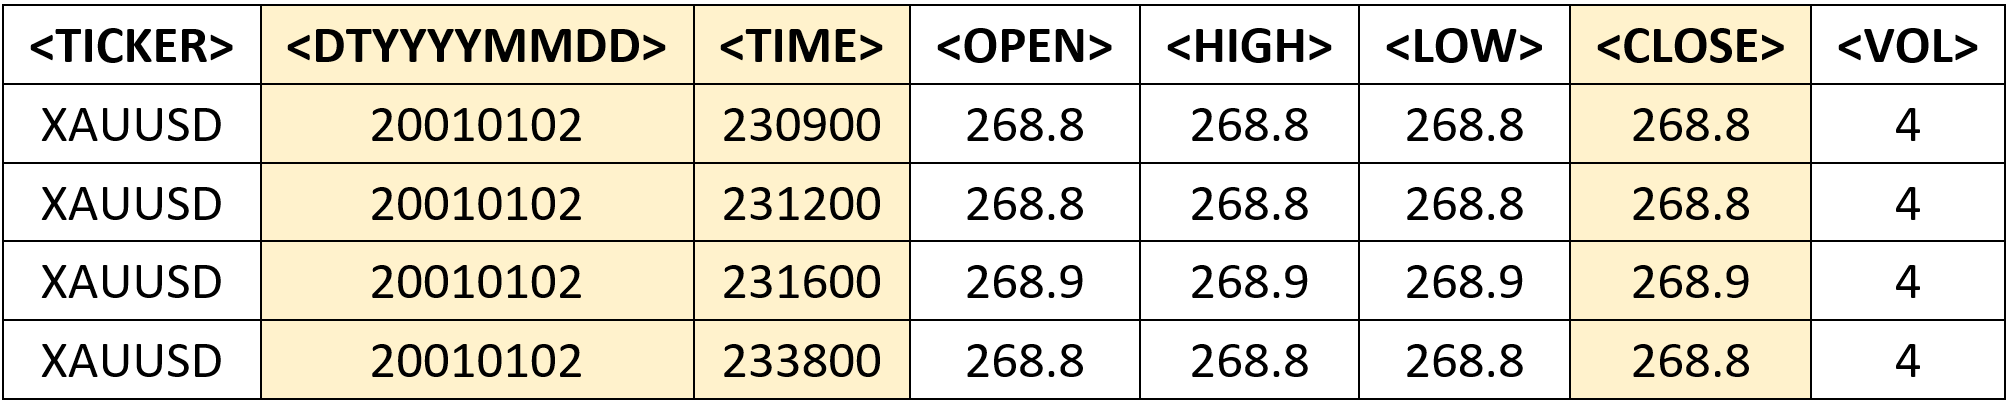
\includegraphics[width=5.5in]{4.jpg}

\H{Sample 3:}

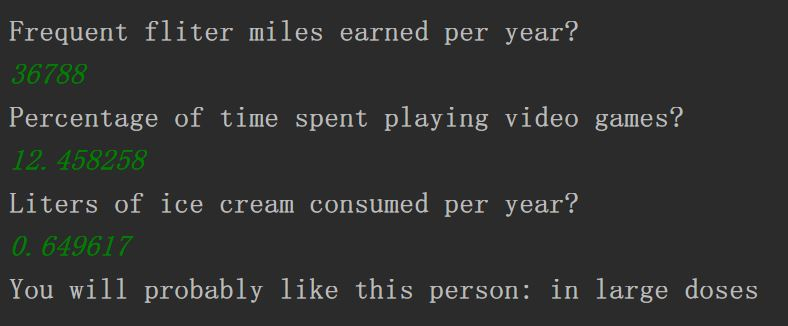
\includegraphics[width=5.5in]{7.jpg}

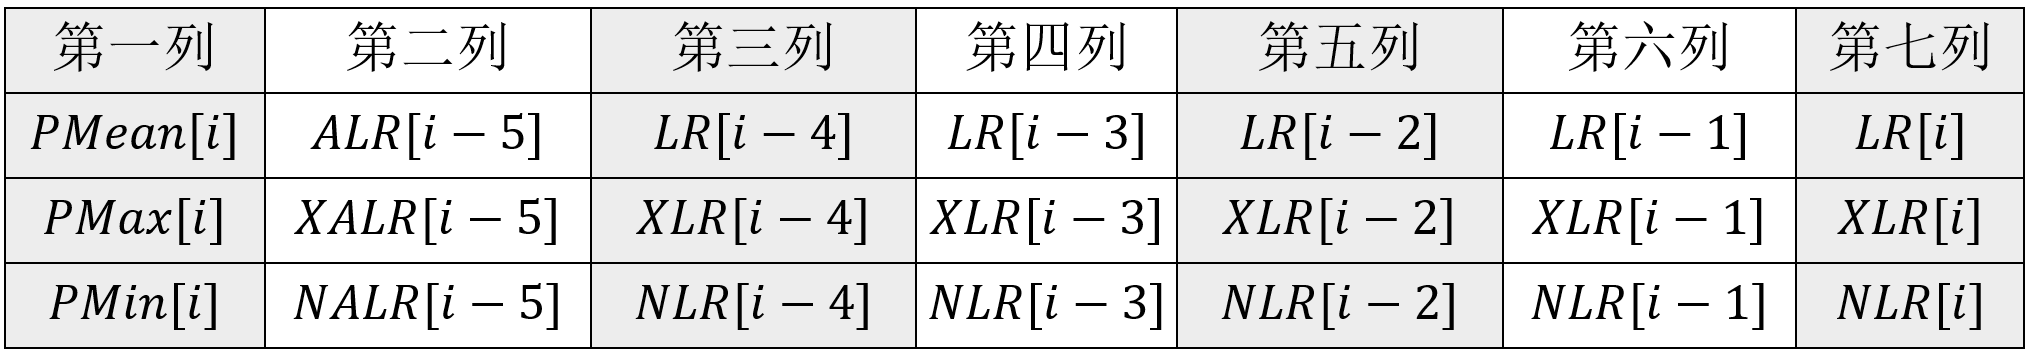
\includegraphics[width=5.5in]{6.jpg}

It works not bad! It took me much time to draw the picture in different colors by using "matplotlib.py", and I think it's a pretty good tool for me. And I have decided to spend more time on learning it.

\section{\H 外汇与汇率}
\subsection{\H 外汇、汇率的概念}
\subsubsection{外汇}
外汇是国际汇兑的简称。它有动态和静态之分。动态意义上的外汇,是指经过银行等金融机构把一国货币兑换成另一国货币的行为。静态意义上的外汇,是指以外币表示的,可用于国际结算的支付手段。
\subsubsection{汇率}
汇率是指一国货币兑换成另一国货币的比率。对一国而言,汇率即本币和外币之间的兑换比率。在外汇市场上,汇率又常常被称为汇价、外汇行情或外汇市行市。

\subsection{\H 汇率的决定及其变动}
\subsubsection{汇率的决定的基础}
汇率作为不同货币之间的兑换比率,其决定的基础是国际金融学研究的核心理论之一。

1.汇率决定的直接基础

1)金本位制度下汇率决定的直接基础

金本位货币制度是以黄金作为本位货币的一种货币制度,包括金币本位制、金块本位制和金汇兑本位制。金币本位制是典型的金本位制,金块本位制和金汇兑本位制是削弱了的、没有金币流通的金本位制。通常,金本位制度主要是制金币本位制。

在金币本位制度下,各国都规定了每一金铸币单位包含的黄金重量与成色,即含金量。在这种制度下,两国货币间的比价要用他们各自包含的含金量来折算。因此,含金量是决定两国货币汇率的直接基础。两种货币含量的对比叫铸币平价。因此,也可以说铸币平价是决定两种货币汇率的直接基础。

在外汇市场上,由于受外汇供求关系的影响,汇率行市有时高于、有时低于铸币平价。当某种货币供过于求时,该货币的汇率就会跌到铸币平价以下,当求大于供时,该货币汇率就会上升到铸币平价以上。

2)纸币流通下汇率决定的直接基础

在纸币流通情况下,如果纸币真正代表所规定的黄金平价时,则两种货币的黄金平价之比,是决定汇率的直接基础。两种货币的汇率则是围绕着黄金平价并受外汇供求影响上下波动。

然而,纸币由于不能与黄金兑换,又没有储藏手段的职能,所以在纸币发行量过大时,通货膨胀就会发生。在这种情况下,汇率决定的直接基础就不是纸币的黄金平价,而应是纸币实际代表的金量。一旦纸币实际所代表的含金量与名义上规定的含金量相差太远,以至于是各国中央银行难以用有限的外汇平准基金来干预外汇市场,并使汇率稳定在规定的限度之内时,各国政府就会宣布本国纸币的贬值或者升值。

在纸币具有法定含量的纸币流通时期,汇率决定的情况在“二战”后布雷顿森林货币体系中得到充分体现。各国通过协商,在各自单位纸币法定含金量基础上确定各国货币与美元的固定比价,并规定汇率波动的限度,如果超过这个限度,各国政府负责干预管理或实行法定的升值或贬值。因此,此时期汇率基本稳定,波动不大,故也成为固定汇率制。

布雷顿森林国际货币制度崩溃以后,各国普遍实行浮动汇率制,政府不再规定货币的含金量。如果国内物价上涨,货币的对内购买力下降,而汇率仍保持不变,则表明高估本币的对外价值。本币比值的长期高估必然影响本国的国际收支,经过一段时间,就必须调整到与国内购买力基本一致的水平。两种货币购买能力的对比,叫购买力平价。所以,也可以说购买力平价是在纸币不规定含量的纸币本位制度下汇率决定的直接基础。购买力强的货币汇率就高,购买力弱的货币汇率就低,汇率浮动随行就市,不再有波动的界限,因此成为浮动汇率制。

2、汇率决定的最终基础

研究汇率决定的基础,仅仅看到它的直接基础,在理论上是不彻底的。因此,还必须分析这些直接基础背后的决定因素。这种背后的决定因素就是货币具有的或所代表的价值。价值量是汇率决定的最终基础。不同国家的货币之间之所以有比值是因为他们有可比性。各种货币的可比性来自于货币本身具有的价值或所能代表的价值。因此,两种货币所具有或所代表的价值之比就是汇率决定的最终基础。

\subsubsection{影响汇率变动的因素}
\paragraph{\H 经济增长率}
经济增长率比较高,说明改过经济发展比较快,经济实力在增强,投资利润率高,出口旺盛,改过货币稳定,这会加强外汇市场上人们对该国货币的信心,该国货币的汇率一般会呈上升趋势。
\paragraph{\H 国际收支状况}
一国国际收支持续顺差,外汇收入增多,国际储备随之增加,外汇市场对该国货币的需求增加,必然推动该国货币币值的上浮,使该国货币成为世界上的强势货币或者硬货币。
\paragraph{\H 通货膨胀}
在通货膨胀条件下,货币购买力会下降,两国通货膨胀率的差异必然导致汇率发生变动。比如,甲国的通货膨胀率超过乙国,甲国的货币汇率就会下降。通货膨胀对汇率的影响,一般要经过一段时间(比如半年甚至更长时间)才能表现出来。
\paragraph{\H 利率水平}
利率的高低,决定投资者的收益水平。在各国货币利率出现差异时,投资者必然将短期资金从低利率货币兑换成高利率货币,并投放到收益大的国家去,这势必带来国际金融市场上不同货币的供求变动,从而影响汇率的变动。一般来说,一国利率提高,可吸引大量资本流入,促使本币汇率上升,外汇汇率相对下跌。一国利率降低,会促使大量资本外流,本币汇率下降,外汇汇率上升。



%%****************************************
%%  参考文献
%%****************************************
\bibliography{myreference}
\bibliographystyle{plain}
\end{document}  
